%!TEX program = lualatex
\documentclass[aspectratio=169,11pt]{beamer}

% ===== Tema =====
\usetheme{Madrid}
\usecolortheme{whale}
\setbeamertemplate{navigation symbols}{}

% ===== Idioma =====
\usepackage[portuguese]{babel}

% ===== Fonte =====
\usepackage{fontspec}
\setmainfont{Latin Modern Roman}

% ===== Figuras / tabelas =====
\usepackage{graphicx}
\usepackage{booktabs}
\usepackage{siunitx}

% ===== URLs =====
\usepackage{xurl}

% ===== TikZ / watermark =====
\usepackage{tikz}
\usetikzlibrary{calc}

% ===== Referências =====
\usepackage[style=abnt, backend=biber]{biblatex}
\usepackage{csquotes}
\addbibresource{referencias.bib}

% ===== Logo =====
\titlegraphic{
\includegraphics[width=1.8cm]{uerj.jpg}}

% ===== Metadados =====
\title[Sem. Cartografia X]{Seminário de Cartografia X}
\subtitle[Aspectos de Atafona]{Caracterização fisiográfica e aspectos oceanográficos de Atafona}
\author[Carneiro, Gaiani e Elsas]{Israel Carneiro \and Miguel Gaiani \and José Mauro Elsas}
\institute[UERJ]{UERJ -- Faculdade de Oceanografia}
\date{abril de 2026}

\begin{document}

% =========================================================
% CAPA
\begin{frame}
\titlepage
\end{frame}

% =========================================================
% SEÇÕES
\section{Objetivo}
\section{Caracterização Fisiográfica}
\section{Metodologia}
\section{Discussão}
\section{Conclusão}
\section{Referências}

% =========================================================
% SUMÁRIO
\begin{frame}{Sumário}
\tableofcontents
\end{frame}

% =========================================================
\begin{frame}{Objetivo}
\begin{columns}[T,onlytextwidth]

\begin{column}{0.48\textwidth}
\centering
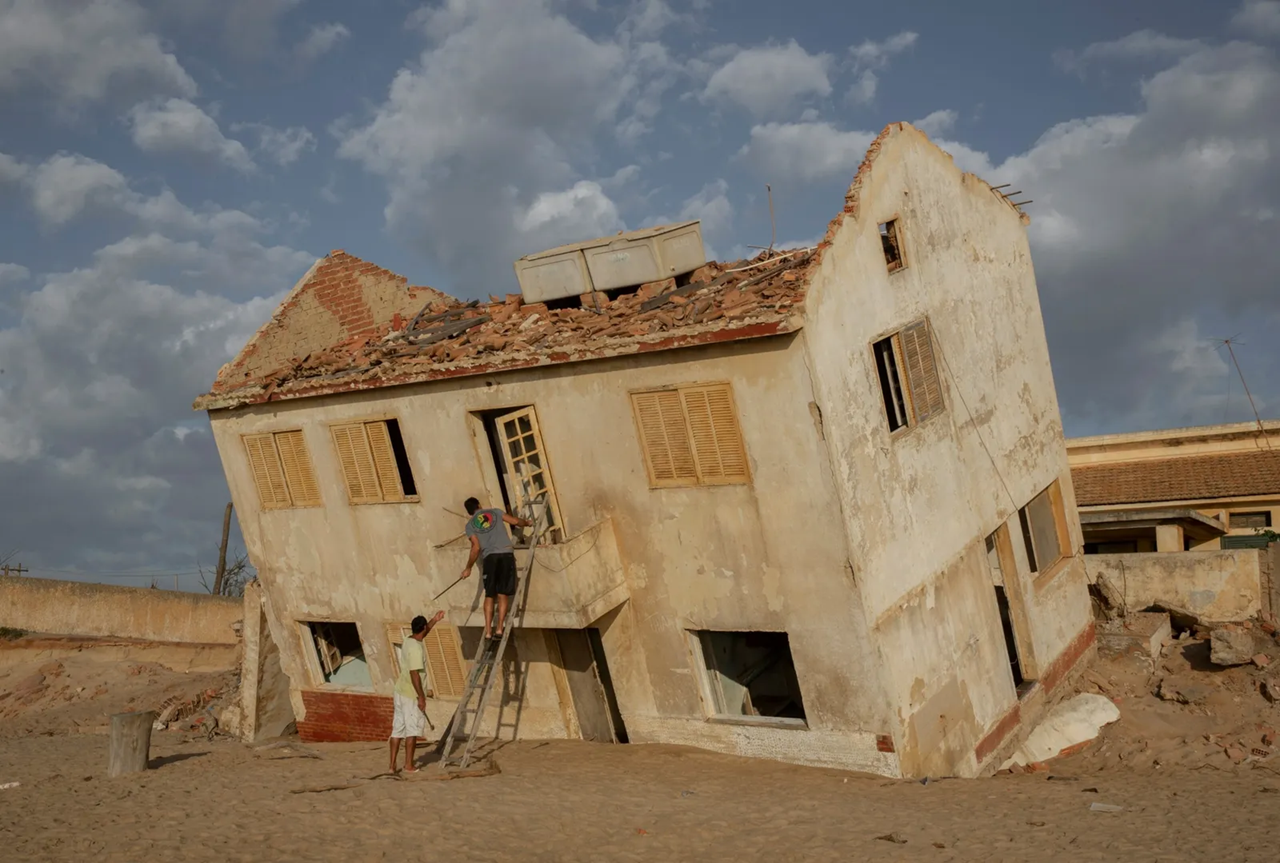
\includegraphics[width=\linewidth,height=0.28\textheight,keepaspectratio]{Atafona_2.png}

\vspace{0.6em}

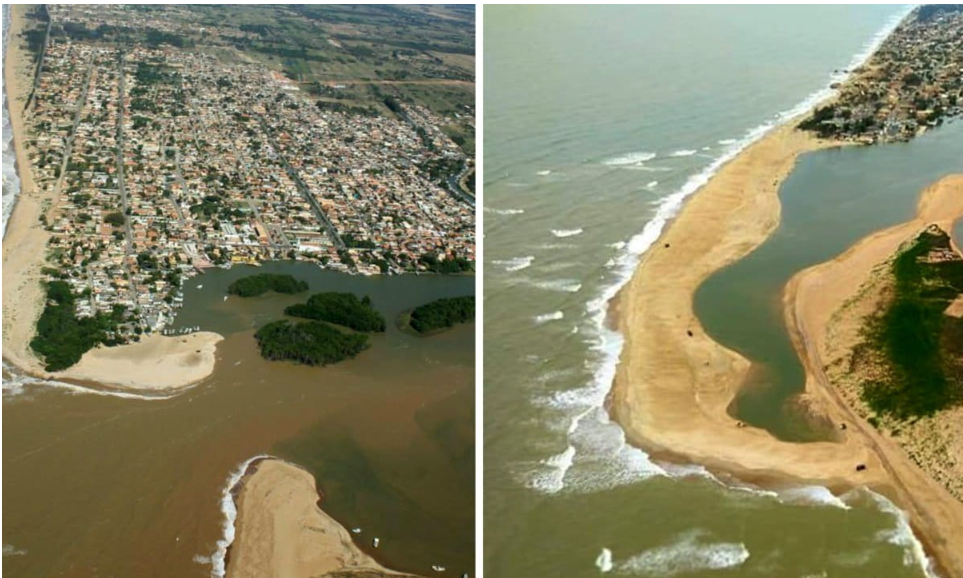
\includegraphics[width=\linewidth,height=0.28\textheight,keepaspectratio]{comparativo_02_19.png}

\vspace{0.3em}
{\small Comparativo entre 2002 e 2019.}

{\tiny Fonte: \cite{briso_atafona_2021}}
\end{column}

\begin{column}{0.48\textwidth}
\begin{itemize}
    \item Identificar as causas da erosão costeira em Atafona e o desequilíbrio entre processos fluviais e marinhos.

    \item Avaliar a hipótese de alteração do equilíbrio hidrossedimentar na foz do rio Paraíba do Sul.

    \item Propor medidas de mitigação frente à erosão da linha de costa que atinge Atafona há muitos anos.
\end{itemize}
\end{column}

\end{columns}
\end{frame}

% =========================================================
\begin{frame}{Caracterização fisiográfica I}
\begin{columns}[T,onlytextwidth]

\begin{column}{0.48\textwidth}
A região de Atafona, localizada em São João da Barra, no delta do rio Paraíba do Sul, apresenta:

\begin{itemize}
    \item ambiente costeiro e fluviodeltaico de baixa altitude;
    \item planície costeira e deltaica composta por sedimentos inconsolidados;
    \item predomínio de areias, siltes e argilas.
\end{itemize}

{\small O delta do Paraíba do Sul também é uma área de intensa mineração de areia.}
\end{column}

\begin{column}{0.48\textwidth}
\centering
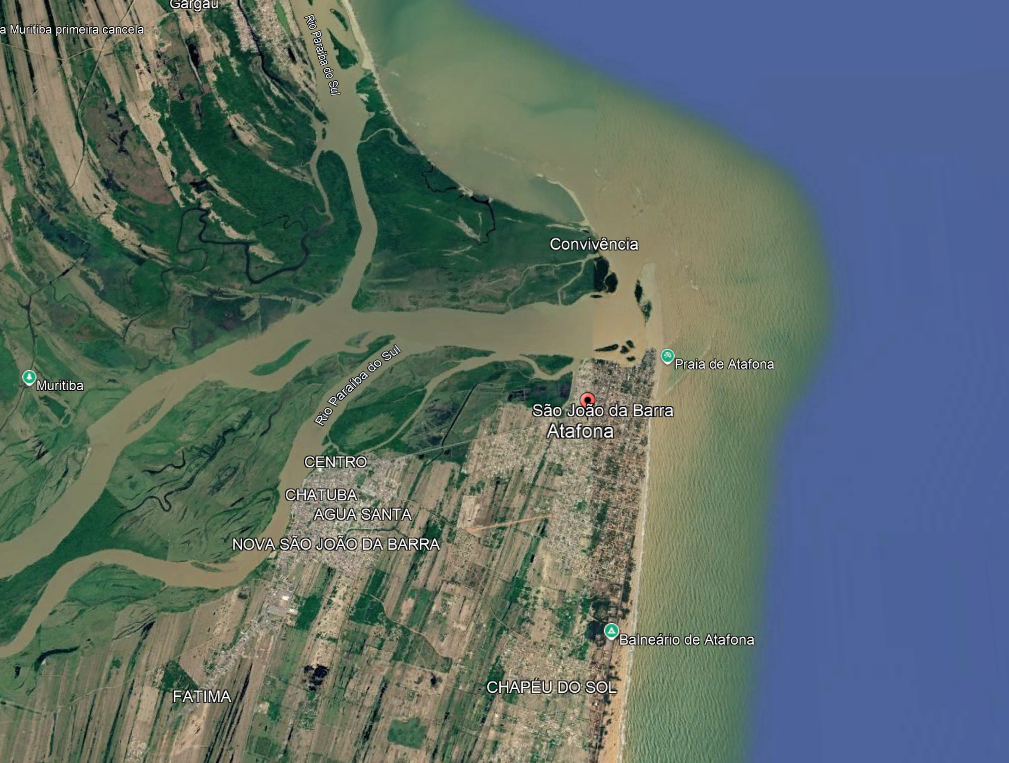
\includegraphics[width=\linewidth,height=0.7\textheight,keepaspectratio]{Atafona_1.png}

\vspace{0.3em}
{\footnotesize Atafona, São João da Barra}
\end{column}

\end{columns}
\end{frame}

% =========================================================
\begin{frame}{Caracterização fisiográfica II}
\begin{columns}[T,onlytextwidth]

\begin{column}{0.48\textwidth}
\centering
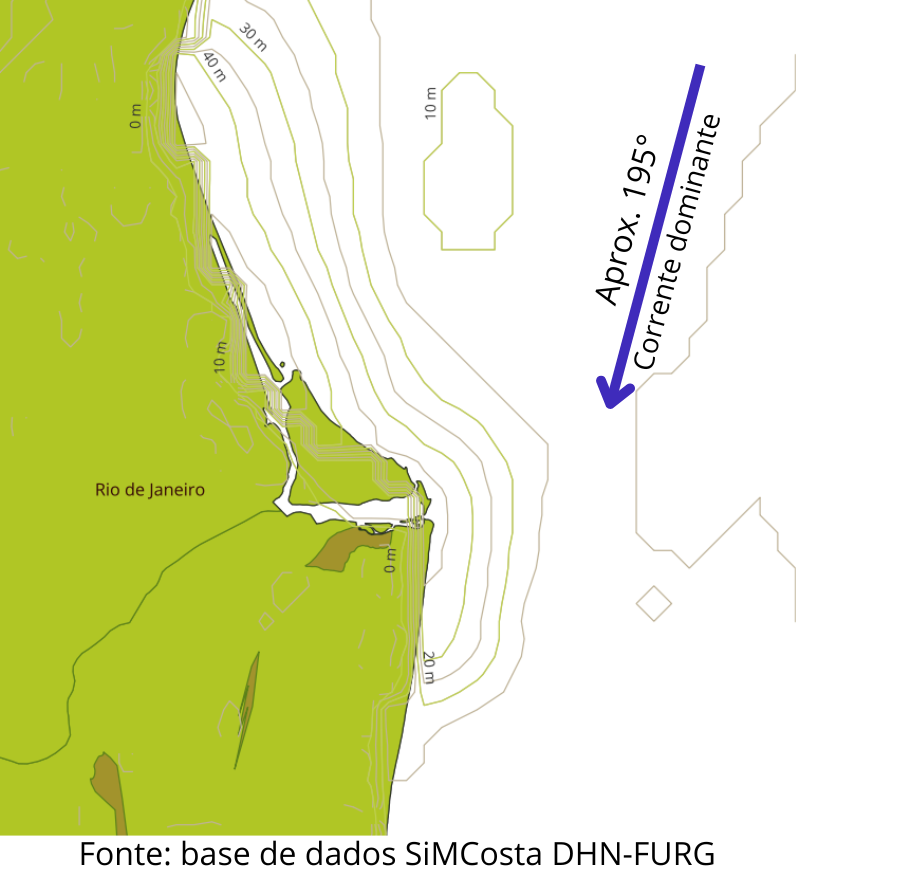
\includegraphics[width=\linewidth,height=0.7\textheight,keepaspectratio]{Aprox_195graus.png}

\vspace{0.3em}
{\footnotesize Batimetria em Atafona, São João da Barra}
\end{column}

\begin{column}{0.48\textwidth}
A dinâmica da região resulta da interação entre processos:

\begin{itemize}
    \item fluviais, associados à descarga e ao transporte sedimentar;
    \item marinhos, associados às ondas e correntes;
    \item atmosféricos, associados aos ventos com base em \cite{vasconcelos2021_atafona_grussai}
\end{itemize}

Essa interação confere elevada mobilidade morfológica, favorecendo a erosão costeira.

{\small Destaca-se o papel do equilíbrio morfodinâmico na região do delta.}
\end{column}
\end{columns}
\end{frame}


% =========================================================
\begin{frame}{Metodologia I}
\begin{columns}[T,onlytextwidth]
\begin{column}{0.48\textwidth}
A metodologia consiste na análise de:

\begin{itemize}
    \item mapas batimétricos;
    \item imagens de satélite;
    \item material cartográfico;
    \item Base de dados de direção e velocidade de corrente medida por ADCP (\emph{Acoustic Doppler Current Profiler}). \cite{simcosta_dados_2026}
\end{itemize}

\end{column}

\begin{column}{0.48\textwidth}
\centering
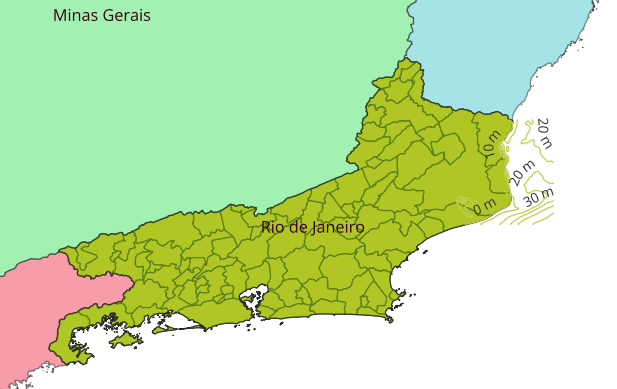
\includegraphics[width=\linewidth,height=0.7\textheight,keepaspectratio]{rj_regiao.png}

\vspace{0.3em}
{\footnotesize Litoral norte do Rio de Janeiro}
\end{column}

\end{columns}
\end{frame}

% =========================================================
\begin{frame}{Metodologia II}
\begin{columns}[T,onlytextwidth]


\begin{column}{0.48\textwidth}
\centering
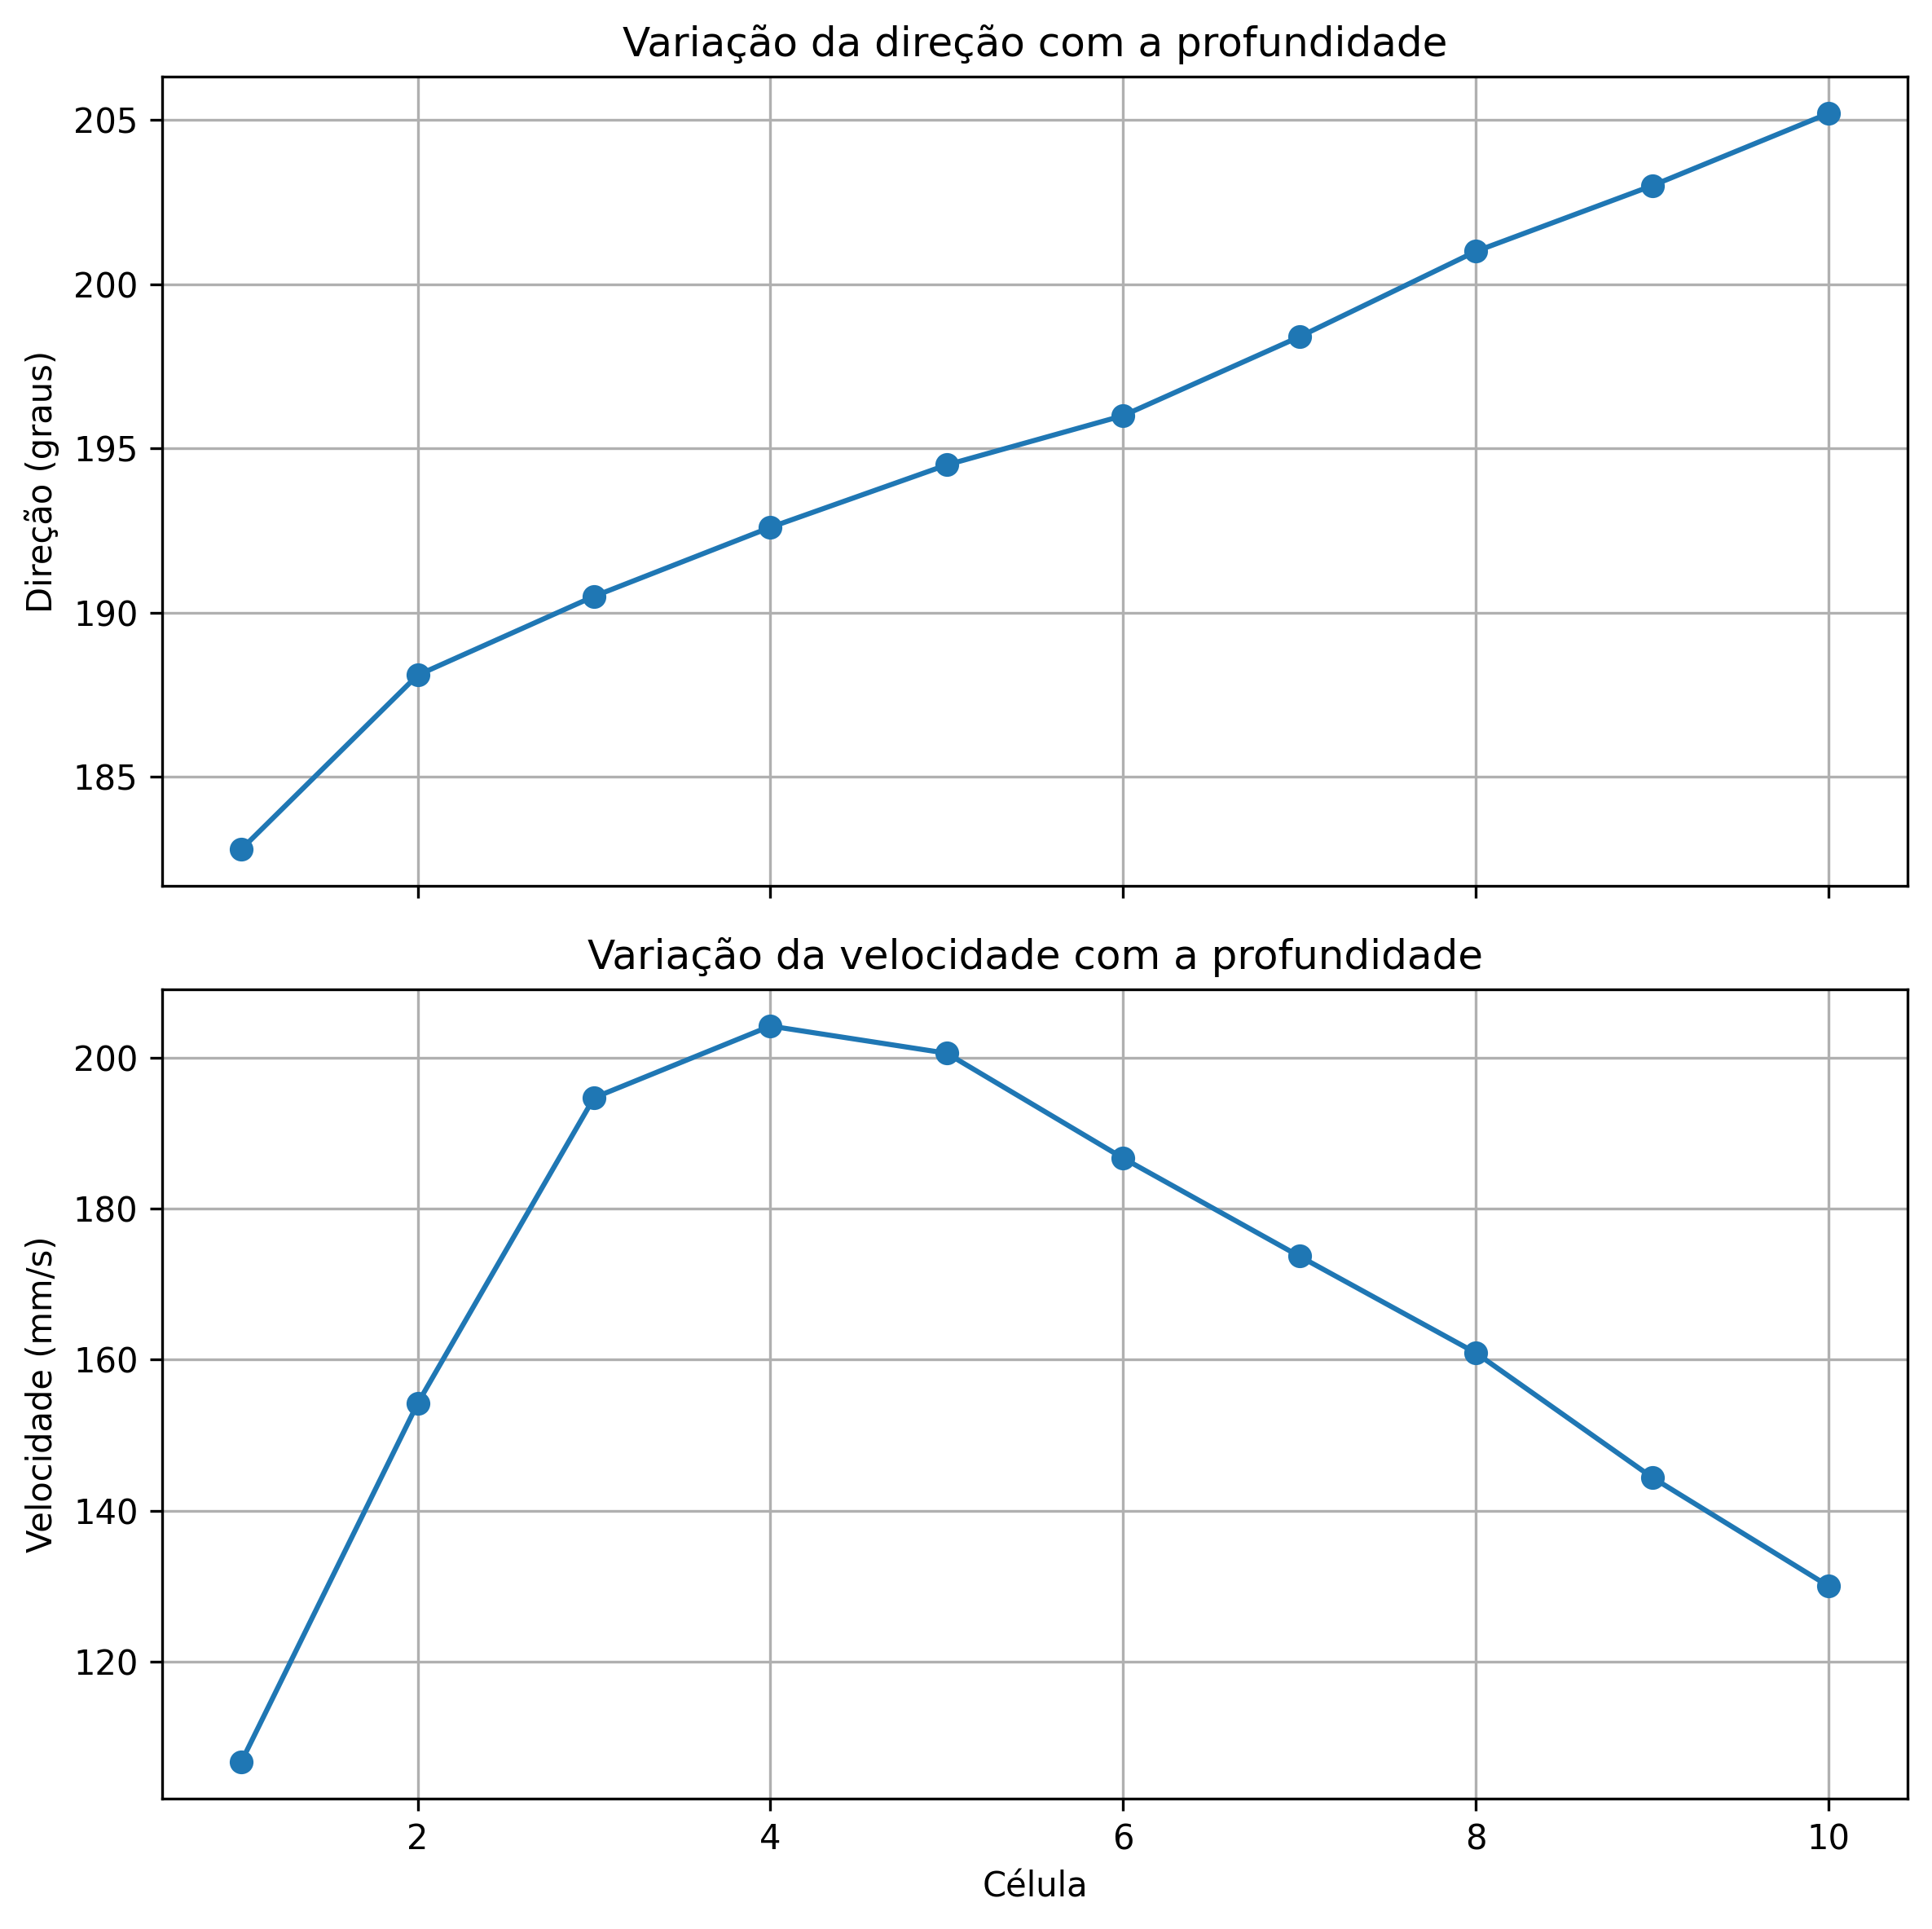
\includegraphics[width=\linewidth,height=0.7\textheight,keepaspectratio]{direcao_velocidade_cells.png}

\vspace{0.3em}
{\footnotesize Litoral norte do Rio de Janeiro}
\end{column}

\begin{column}{0.48\textwidth}
    \vspace{3em}
Para a análise de corrente temos:

\begin{itemize}
    \item Coordenadas: lat.= -19.69518331 lon = -39.77213332,
    \item Equipamento: Nortek Aquadopp Profiler 600kHz
    \item A análise foi feita com 10 células,
    \item O vetor representativo é \SI{0.165}{\meter\per\second} azimute \SI{195}{\degree}
\end{itemize}

\end{column}

\end{columns}
\end{frame}


% =========================================================
\begin{frame}{Discussão e resultados I}
\begin{columns}[T,onlytextwidth]

\begin{column}{0.48\textwidth}
    \vspace{3em}
\begin{itemize}
    \item Reduções na vazão do rio Paraíba do Sul, associadas a intervenções antrópicas, diminuíram o aporte sedimentar e favoreceram o avanço da cunha salina;
    \item Intensificação dos processos erosivos na região de Atafona.
    \item Observa-se erosão costeira intensa e recuo significativo da linha de costa em Atafona.
\end{itemize}

\end{column}

\begin{column}{0.48\textwidth}
\centering
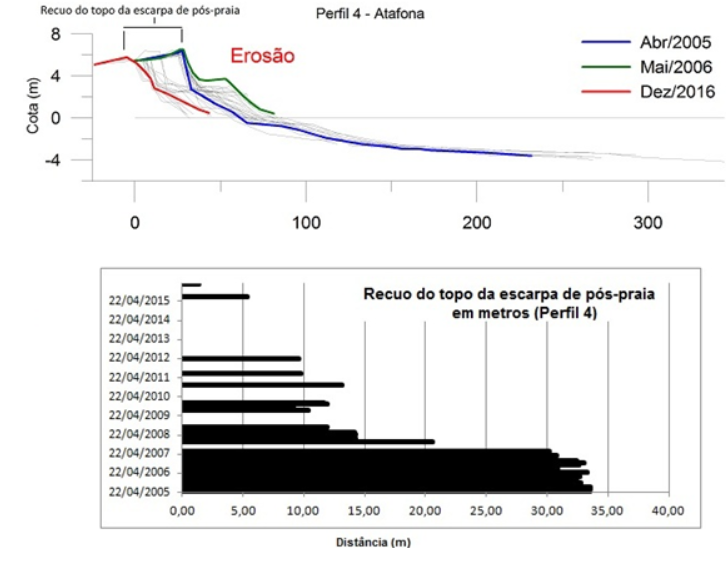
\includegraphics[width=\linewidth,height=0.7\textheight,keepaspectratio]{avanço_erosão.png}

\vspace{0.3em}
{\footnotesize Avanço da erosão em Atafona}\\
\cite{mello2018_erosao_atafona}
\end{column}

\end{columns}
\end{frame}
% =========================================================
\begin{frame}{Discussão e resultados II}
\begin{columns}[T]
    \begin{column}{0.48\textwidth}
        \centering
        \vspace{2em}
        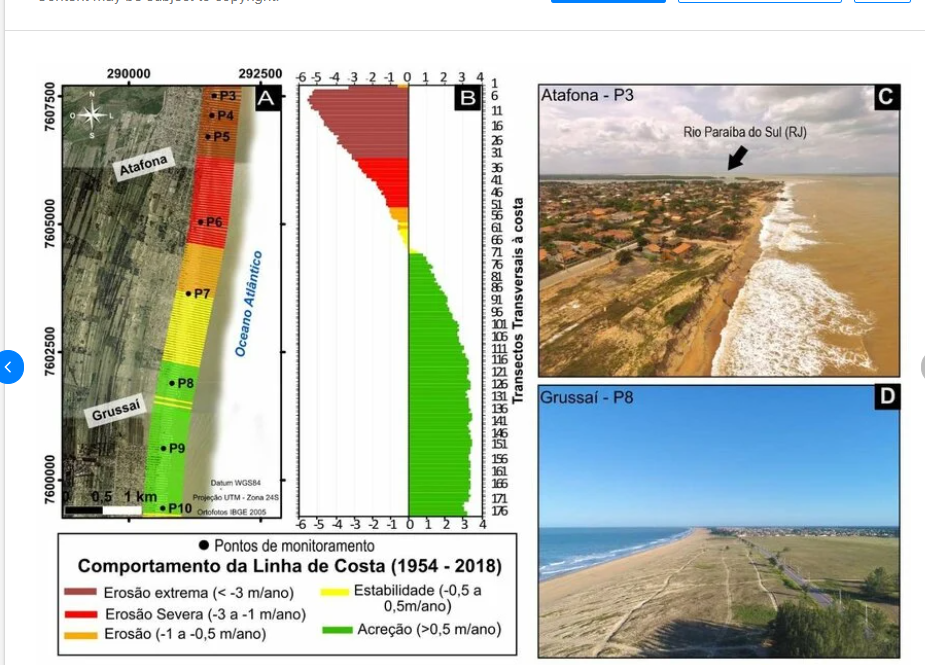
\includegraphics[width=\linewidth]{atafona_grussai.png}
        
        \vspace{0.2cm}
        \footnotesize Fonte: \cite{machado2024_dinamica_linha_costa_paraiba_sul}
    \end{column}

    \begin{column}{0.48\textwidth}
        \begin{itemize}
    \item Em um sistema de baixa altitude e sedimentos inconsolidados, pequenas alterações no balanço sedimentar podem produzir respostas geomorfológicas expressivas.

    \item Esse comportamento é consistente com estudos recentes sobre a dinâmica costeira em Atafona. \cite{vasconcelos2021_atafona_grussai}

    \item A direção predominante das correntes (\(\approx 195^\circ\)) sugere transporte longitudinal de sedimentos, contribuindo para a remoção de material da região deltaica.
        \end{itemize}
    \end{column}
\end{columns}
\end{frame}

% =========================================================
\begin{frame}{Discussão e resultados III}
\begin{columns}[T,onlytextwidth]
    \begin{column}{0.48\textwidth}
        \centering
        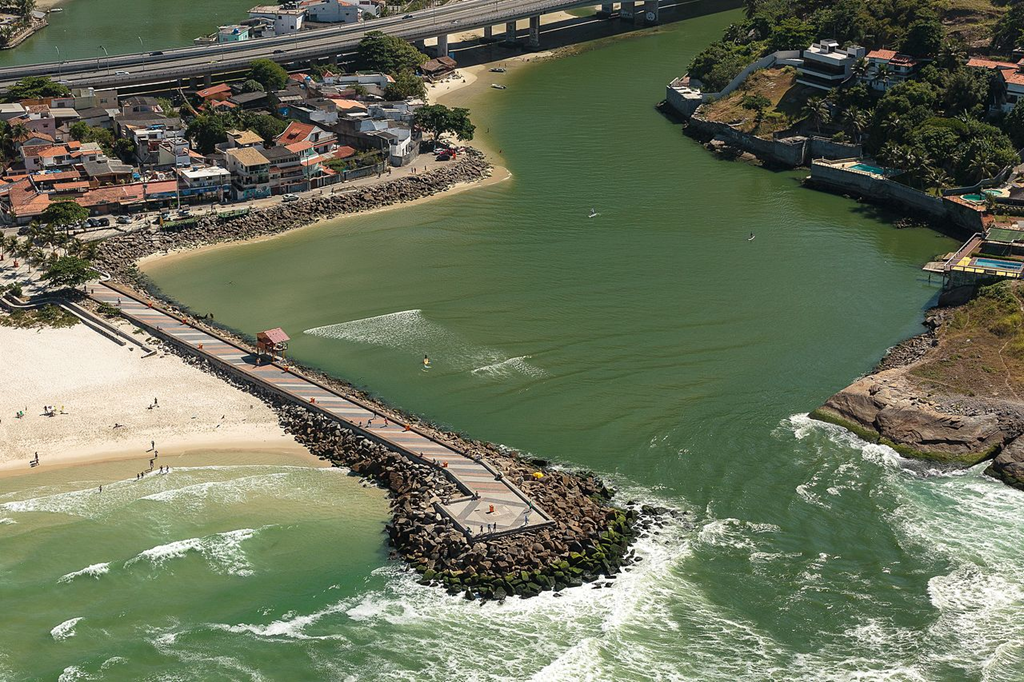
\includegraphics[width=\linewidth]{quebra_mar.png}
        \vspace{0.3em}
        {\footnotesize Quebra-mar, Barra da Tijuca, Rio de Janeiro.}\\
        {\tiny \cite{wiki_marpedia_quebra}}
    \end{column}

    \begin{column}{0.48\textwidth}
        \begin{itemize}
            \item Construção de estruturas de proteção costeira, como quebra-mares, para reduzir a energia das ondas incidente na faixa litorânea.

            \item Monitoramento contínuo da dinâmica costeira e da vazão do rio Paraíba do Sul, a fim de compreender a evolução do desequilíbrio hidrossedimentar.

            \item Desenvolvimento de estratégias integradas de gestão costeira, considerando fatores fluviais, marinhos e antrópicos.
        \end{itemize}
    \end{column}
\end{columns}
\end{frame}

% =========================================================
\begin{frame}{Discussão e resultados IV}
\begin{columns}[T]
    \begin{column}{0.48\textwidth}
        \centering
        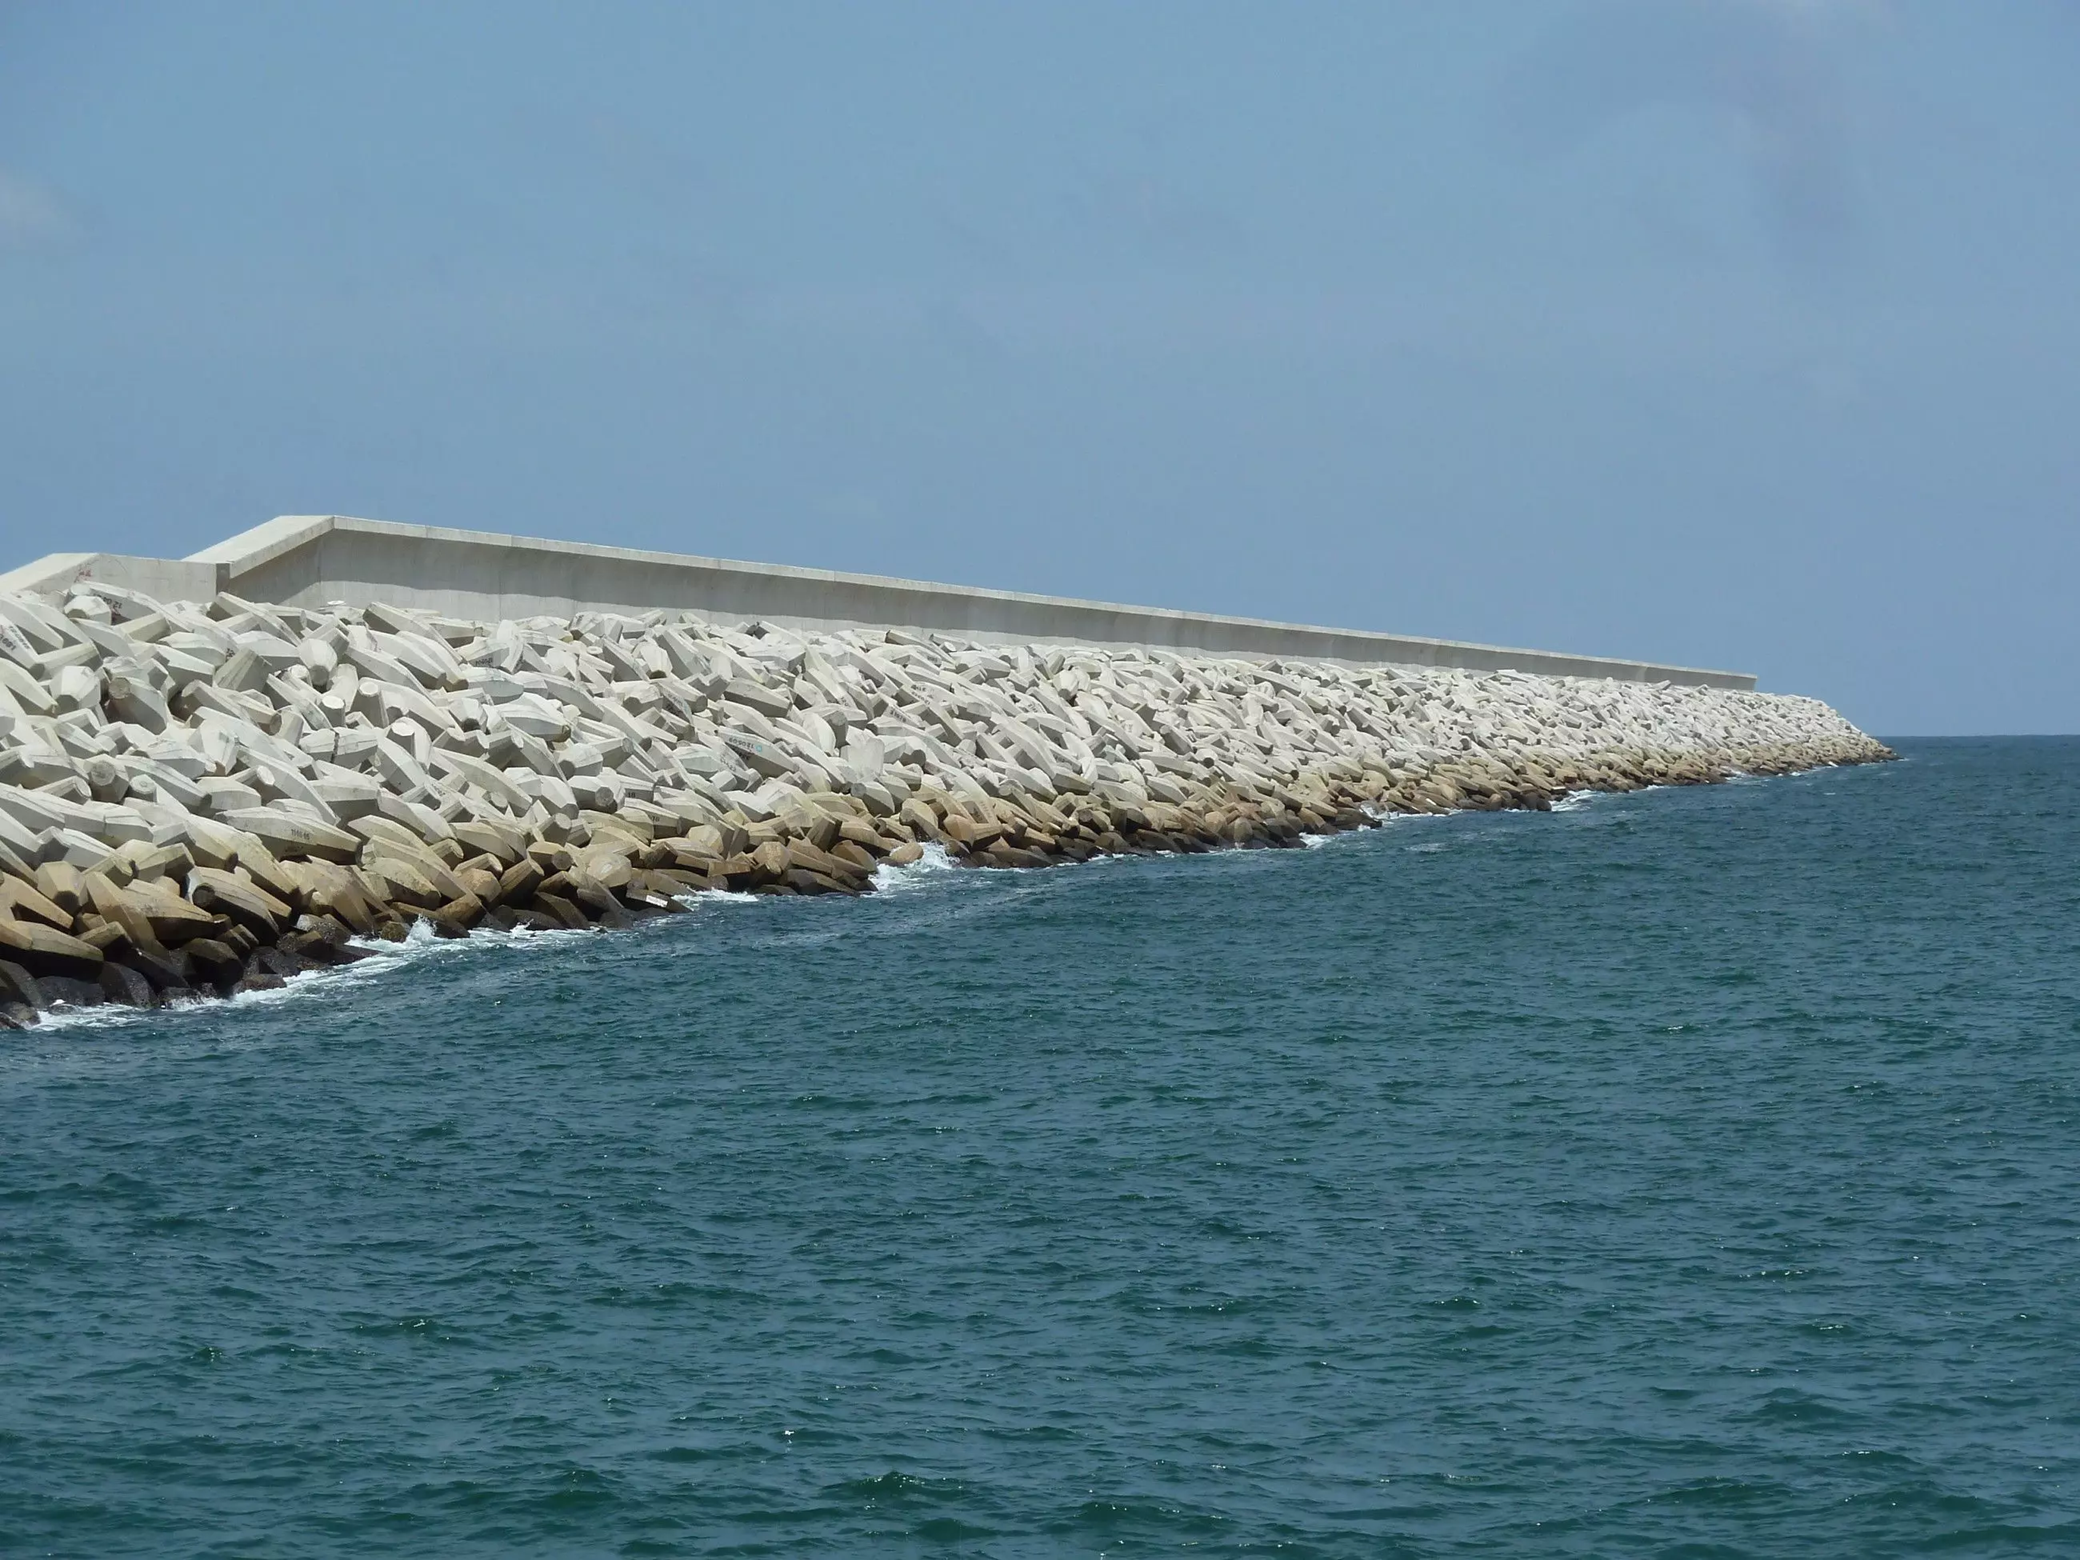
\includegraphics[width=\linewidth,height=0.72\textheight,keepaspectratio]{Core-loc_break_water.png}
        
        \vspace{0.15cm}
        \footnotesize Quebra-mar em Core-Locs\texttrademark
    \end{column}

    \begin{column}{0.48\textwidth}
        \begin{itemize}
            \item A redução do aporte sedimentar fluvial tende a favorecer a atuação relativa dos processos marinhos, intensificando a erosão costeira.

            \item Medidas de mitigação, como obras costeiras, poderiam alterar essa dinâmica, embora seus efeitos dependam das condições locais e de avaliação técnica específica.
            
            \item A construção de um quebra-mar com Core-loc\texttrademark\ pode fazer parte da mitigação do problema.
        \end{itemize}
    \end{column}
\end{columns}
\end{frame}

% =========================================================
\begin{frame}{Discussão e resultados V}
\begin{columns}[T]
    \begin{column}{0.48\textwidth}
        \begin{itemize}
            \item O Core-Loc\texttrademark\ é um elemento de proteção que aumenta a estabilidade hidráulica do talude e promove a dissipação da energia das ondas.

            \item Cada unidade é georreferenciada com o uso de Estação Total, DGPS e (Real-Time Kinematics) RTK, o que garante que a obra seguirá muito de perto o projeto geomorfológico.

            \item Ao final da obra um 'as built' é feito e comparado com o projeto, o banco de dados gerado permite comparações futuras.
        \end{itemize}
    \end{column}

    \begin{column}{0.48\textwidth}
        \centering
        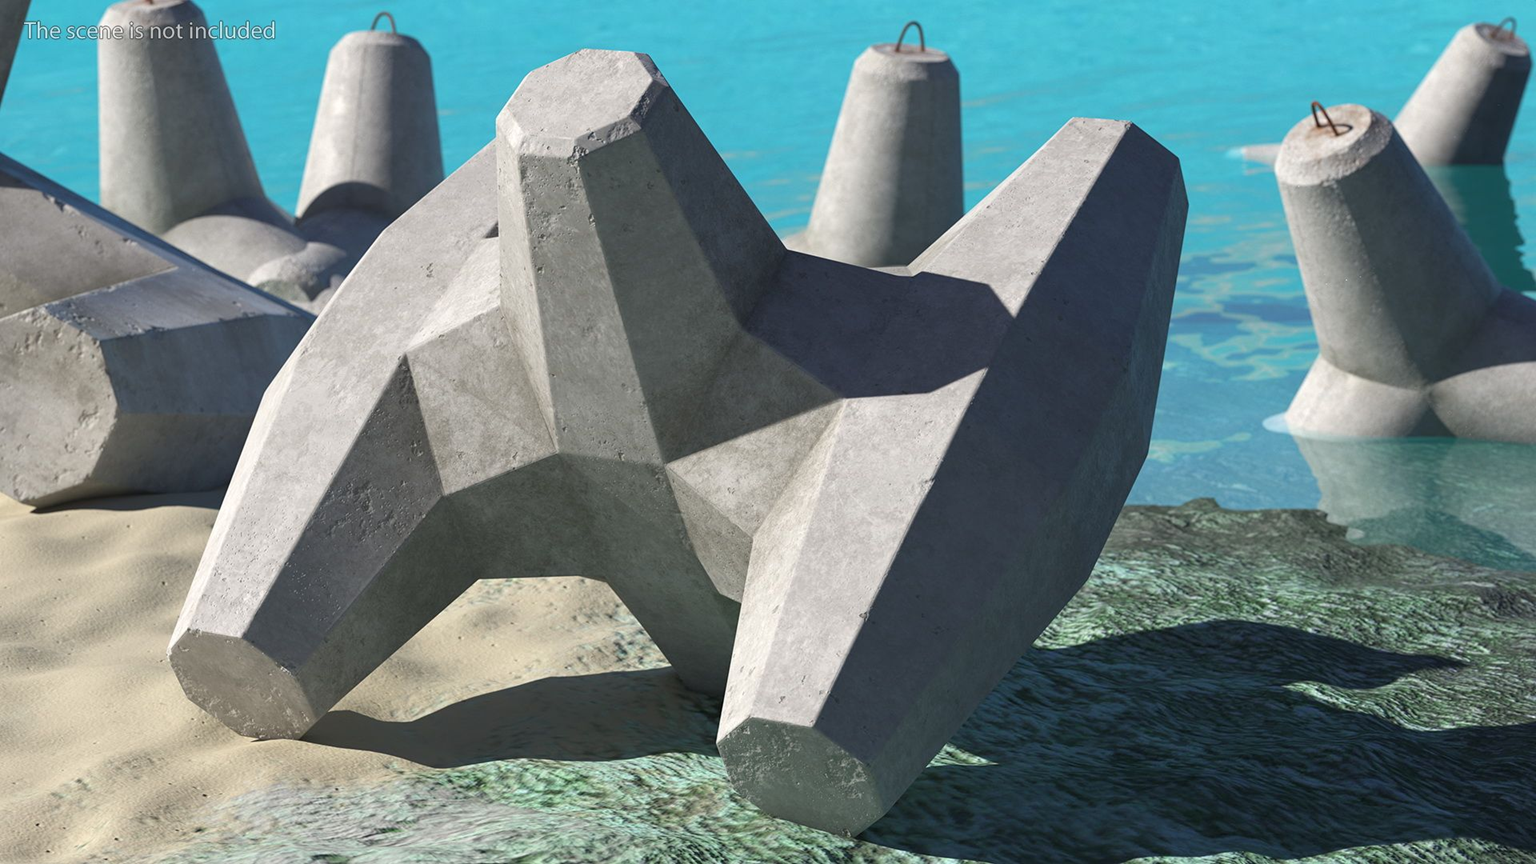
\includegraphics[width=\linewidth,height=0.72\textheight,keepaspectratio]{core_loc_3d.png}
        
        \vspace{0.15cm}
        \footnotesize Fonte: \cite{cli_coreloc}.
    \end{column}
\end{columns}
\end{frame}
% =========================================================%
\begin{frame}{Conclusões I}
\begin{columns}[T]
    \begin{column}{0.48\textwidth}
        \centering
        \vspace{3em}
        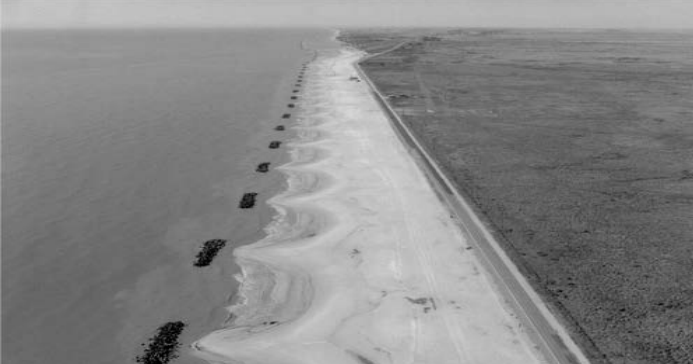
\includegraphics[width=\linewidth,height=0.72\textheight,keepaspectratio]{Holly_beach.png}
        
        \vspace{0.15cm}
        \footnotesize Fonte: \cite{asbpa2011_erosion_control_structures}.
    \end{column}

    \begin{column}{0.48\textwidth}
        \begin{itemize}
            \item Há casos de sucesso no uso de estruturas, como em Holly Beach, Louisiana, no Golfo do México, onde foram instaladas estruturas ao longo do litoral. Essas estruturas contribuíram para mitigar os efeitos da erosão.

            \item Projetos compatíveis com a dinâmica local têm boas chances de reduzir o problema.

            \item O monitoramento contínuo e a avaliação técnica específica servirão para evitar a transferência do problema para áreas adjacentes.
        \end{itemize}
    \end{column}
\end{columns}
\end{frame}

% =========================================================
\begin{frame}{Conclusões II}
\begin{columns}[T]
    \begin{column}{0.48\textwidth}
        \begin{itemize}
            \item Independentemente do tipo de material utilizado (blocos naturais ou unidades artificiais como Core-Loc\texttrademark), diferentes configurações geométricas de estruturas costeiras têm sido empregadas com sucesso; 

\item Em (a), observam-se espigões em configuração típica.
\item Em (b), observa-se um arranjo típico de quebra-mares ao longo da praia.

        \end{itemize}
    \end{column}

    \begin{column}{0.48\textwidth}
        \centering
        \vspace{2em}
        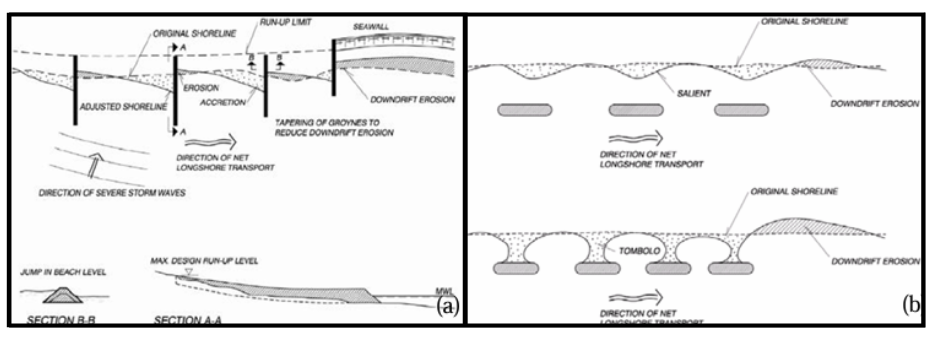
\includegraphics[width=\linewidth,height=0.72\textheight,keepaspectratio]{Figs_a_b.png}
        \vspace{0.15cm}
        \footnotesize Fonte: \cite{asbpa2011_erosion_control_structures}.
    \end{column}
\end{columns}
\end{frame}

% =========================================================
\begin{frame}{Conclusões III}
\begin{columns}[T]

    \begin{column}{0.48\textwidth}
        \centering
        \vspace{4em}
        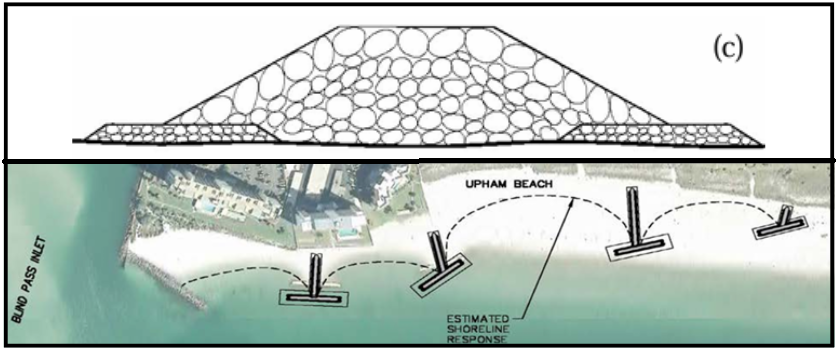
\includegraphics[width=\linewidth,height=0.72\textheight,keepaspectratio]{Figs_c_d.png}
        \vspace{0.15cm}
        \footnotesize Fonte: \cite{asbpa2011_erosion_control_structures}.
    \end{column}

        \begin{column}{0.48\textwidth}
            \vspace{1em}
        \begin{itemize}
            \item Complementando:

            \item em (c) vemos a seção transversal de um quebra-mar.

\item Em (d), observa-se a resposta prevista da linha de costa para espigões em T em \emph{Upham Beach, Florida}.
\item A linha tracejada representa a posição projetada de equilíbrio morfodinâmico da linha de costa, resultante da alteração do campo de ondas pelas estruturas.
        \end{itemize}
    \end{column}
\end{columns}
\end{frame}

% =========================================================
\begin{frame}[plain]
\begin{tikzpicture}[remember picture,overlay]
\node[opacity=0.18,inner sep=0pt] at (current page.center) {%
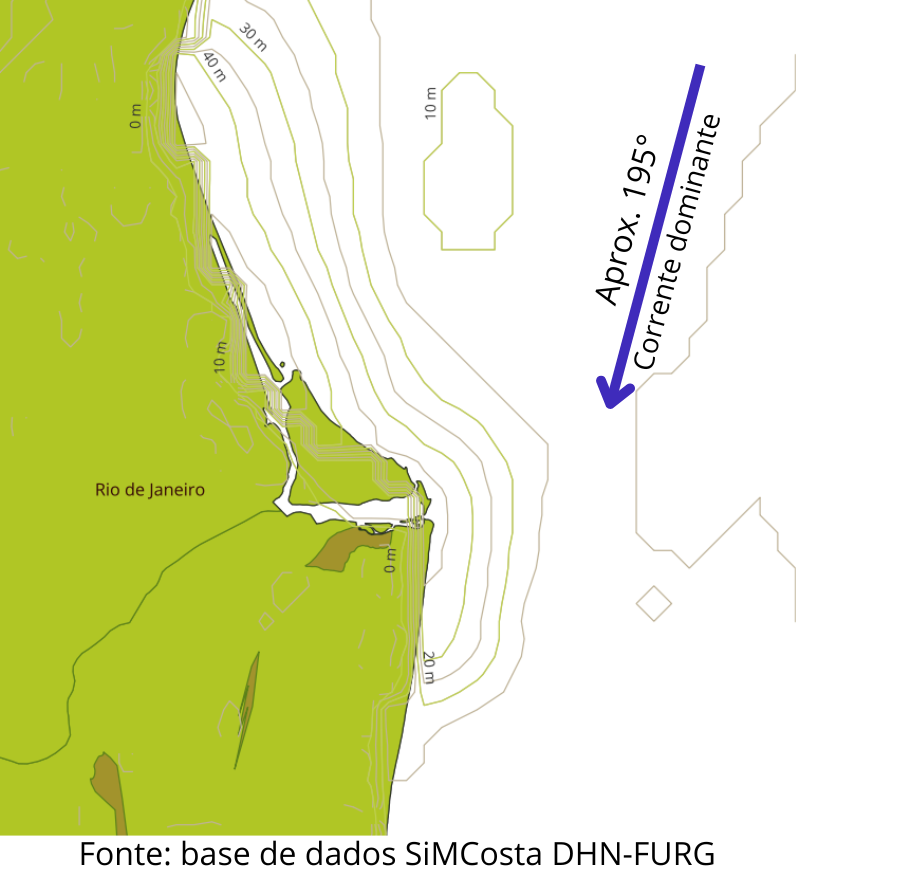
\includegraphics[width=\paperwidth,height=\paperheight]{Aprox_195°.png}};
\end{tikzpicture}

\centering
\vspace*{2.2cm}

{\Huge \textbf{Muito obrigado!}}

\vspace{1.2cm}

{\Large Perguntas?}

\vfill

{\footnotesize Nosso Grupo\\
UERJ -- Faculdade de Oceanografia}

\vspace{0.6cm}
\end{frame}
% =========================================================

\nocite{briso_atafona_2021}

\begin{frame}[allowframebreaks]{Referências}
\scriptsize
\setlength{\bibitemsep}{0pt}
\setlength{\bibhang}{0pt}
\renewcommand*{\bibfont}{\scriptsize}
\printbibliography[heading=none]
\end{frame}

\end{document}